\documentclass[12pt]{article}
\usepackage{amsmath}
\usepackage{amssymb}
\usepackage{geometry}
\usepackage{enumerate}
\usepackage{natbib}
\usepackage{float}%稳定图片位置
\usepackage{graphicx}%画图
\usepackage[english]{babel}
\usepackage{a4wide}
\usepackage{indentfirst}%缩进
\usepackage{enumerate}%加序号
\usepackage{multirow}%合并行
\title{\large UM-SJTU JOINT INSTITUTE\\PHYSICS LABTORATORY\\(VE216)\\\ \\\ \\\ \\\ \\\ \\\ \\\ \\\ \\\ \\\ \\\
LABTORATORY REPORT\\\ \\\ LAB 3\\\ Feedback Control \\\ \\\ \\\ \\\ \\\ }
\author{Name: Pan Chongdan\\ID: 516370910121\\Name Xiang Zhiyuan\\ID: 516370910126}
\date{Date: \today}

\begin{document}
\maketitle
\newpage
\section{Objectives}
\begin{enumerate}
\item Understand feedback control.
\item Build Simple Open Loop Control Plant
\end{enumerate}
\section{Theoretical Background}
\subsection{Preliminary Information}
\subsubsection{A Closed-Loop Feedback Model}	
The block diagram of a generic closed-loop feedback control system is shown in Fig. 1 In this figure,
the “plant” is the system whose output we wish to control. A measurement is performed on the output
by the measurement sub-system, which is then compared with the desired output, i.e., the input to the
control system. The output of the comparator, which computes the difference between the desired and the
actual output, is fed into a controller whose output serves as the input to the plant. If the comparator and
measurement system were removed from the above diagram then one would be left with an open-loop (i.e.,
no feedback) controller.
\begin{figure}[H]
\centering
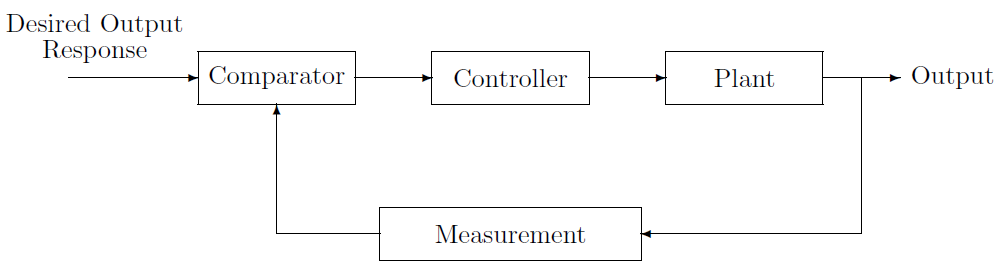
\includegraphics[scale=0.4]{P1.jpg}
\caption{Closed-Loop Control System. The plant is the generic term for the system to be controlled}
\end{figure}
\subsubsection{Closed-Loop Transfer Function}
As mentioned earlier, we will restrict our discussion to the case where all of the blocks shown in Fig. 1
are LTI systems. Thus the input/output relationship of each of these blocks can be described by a system
transfer function. Furthermore, we will realize the comparator as an adder and change the gain on the
measurement to -1. With these changes, the block diagram of Fig. 2 becomes:
\begin{figure}][H]
\centering
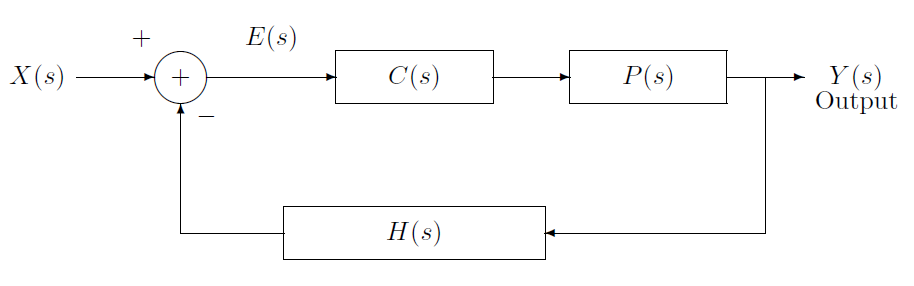
\includegraphics[scale=0.4]{P2.jpg}
\caption{Closed-Loop Feedback Control System.}
\end{figure}
It is a simple matter of algebra to compute the closed-loop transfer function, $G_{cl}(s)=Y(s)/X(s)$, of the
systems shown in Fig. 1 as indicated below.
\begin{equation}
Y(s)=E(s)C(s)P(s)
\end{equation}
\begin{equation}
E(s)=X(s)-H(s)Y(s)
\end{equation}
Combining Eqs. (1) and (2) yields
\begin{equation}
G_{cl}=\frac{Y(s)}{X(s)}=\frac{C(s)P(s)}{1+C(s)P(s)H(s)}
\end{equation}
\begin{equation}
\frac{E(s)}{X(s)}=\frac{1}{1+C(s)P(s)H(s)}
\end{equation}
\subsection{Examples of Feedback Control Systems}
\subsubsection{DC Motor Model}
Let us assume that we want to control the shaft position of a DC motor. To help design a controller for
this DC motor, we mathematically model the angular position, (t) of the shift by the following differential
equation
\begin{equation}
\frac{d^2\theta(t)}{dt^2}+\frac{d\theta(t)}{dt}=V(t)
\end{equation}
where V (t) is the voltage applied to the motor. Thus the plant (i.e., the motor) is a LTI system that has
the following system transfer function
\begin{equation}
P(s)=\frac{1}{s(s+1)}
\end{equation}
This transfer function corresponds to a second-order LTI system with no zeros, and a pair of real poles
located at the origin and at -1.
\subsubsection{No Controller}
Suppose we want the shaft of the motor to rotate by one radian per second by using a unit step as the input, then
\begin{equation}
\theta(s)=V(s)P(s)=\frac{1}{s}\frac{1}{s(s+1)}=-\frac{1}{s}+\frac{1}{s^2}+\frac{1}{s+1}
\end{equation}
where the right-most side of Eq. (5) is obtained by a partial fraction expansion. Consequently,
\begin{equation}
\theta(t)=(t-1+e^{-t})u(t)
\end{equation}
which is clearly not going to achieve the desired rotation by one radian per second!
\subsubsection{Controller Without Feedback}
Shown below is the block diagram of an open-loop controller. We choose a differentiator as the controller,
\begin{figure}[H]
\centering
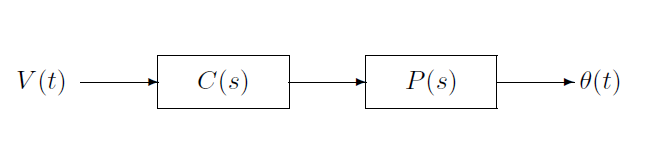
\includegraphics[scale=0.5]{P3.jpg}
\caption{Open-Loop Controller}
\end{figure}
\begin{equation}
C(s)=s
\end{equation}
of a unit-step input. Thus
\begin{equation}
\theta(s)=V(s)C(s)P(s)=\frac{1}{s}s\frac{1}{s(s+1)}=\frac{1}{s}-\frac{1}{s+1}
\end{equation}
Therefore 
\begin{equation}
\theta(t)=(1-e^{-t})u(t)
\end{equation}
Clearly,$\lim_{t\to\inf}\theta(t)=1$, so that this controller results in no steady-state error when the input is a unit step. The response of the DC motor to the unit step, however, is rather slow. It takes approximately 2.3 s for the shaft angle to reach $90\%$ of its final value of 1 radian.
\par We might ask how well this same controller would work if the input were a ramp rather than a step.
Under such circumstances
\begin{equation}
V(s)=\frac{1}{s^2}
\end{equation}
\begin{equation}
\theta(s)=V(s)C(s)P(s)=\frac{1}{s^2}s\frac{1}{s(s+1)}=-\frac{1}{s}+\frac{1}{s^2}+\frac{1}{s+1}
\end{equation}
Therefore
\begin{equation}
\theta(t)=(t-1+e^{-t})u(t)
\end{equation}
and the steady-state error is 1 radian/second. Thus the angular position of the shift deviates from the
desired position by 1 radian as $t\to 1$, and this differentiator-controller is inadequate for a ramp input.
\subsubsection{Sensitivity of an Open-Loop Controller to Plant Changes}
Suppose that overheating changes the transfer function of the mtoro by a small amount to become
\begin{equation}
P(s)=\frac{1}{(s+0.01)(s+1)}
\end{equation}
one of the poles has moved along the real axis from the origin into the left-hand plane (LHP). The step
response of the motor now becomes
\begin{equation}
\theta(s)=V(s)C(s)P(s)=\frac{1}{s}s\frac{1}{(s+0.01)(s+1)}=\frac{100/99}{s+0.01}-\frac{100/99}{s+1}
\end{equation}
Therefore
\begin{equation}
\theta(t)=(100/99)(e^{-0.01t}-e^{-t})u(t)
\end{equation}
and in steady state $\lim_{t\to\inf}=0$, yielding a steady state error of one radian. It is clear that this open-loop
controller is quite sensitive to variations in the plant transfer function.
\subsubsection{Feedback Control}
Consider now the feedback control system shown in Fig. 2 with $H(s)=1,C(s)=Ks$ and $P(s)=1/[s(s+1)]$ as before. Then according to Eq. (3) the closed-loop transfer function
is given by
\begin{equation}
G_{cl}(s)=\frac{Y(s)}{X(s)}=\frac{C(s)P(s)}{1+C(s)P(s)H(s)}=\frac{KsP(s)}{1+KsP(s)}=\frac{K}{s+(K+1)}
\end{equation}
and the step response becomes
\begin{equation}
\theta(s)=V(s)G_{cl}(s)=\frac{1}{s}\frac{K}{s+(K+1)}
\end{equation}
or equivalently
\begin{equation}
\theta(t)=\frac{K}{K+1}(1-e^{-(K+1)t})u(t)
\end{equation}
If $K$ is sufficiently large, then the steady-state error, $lim_{t\to\inf}(V(t)−\theta(t))=1/(K+1)$ will be small. Also
note that the response time is much improved over that obtained by an open-loop controller. In particular,
the 90\% rise-time has been reduced from 2.3 s to 2.3/(K+1)s.
\subsubsection{Sensitivity of the Closed-Loop Controller to Plant Changes}
As before we will consider the situation where the transfer function of the motor changes by a small amount
to become that given by Eq. (15). Using the same feedback controller described above, the closed-loop
response becomes
\begin{equation}
G_{cl}=\frac{Ks}{s^2+(1.01+K)s+0.01}
\end{equation}
Thus the step response is given by
\begin{equation}
\theta(s)=\frac{K}{s^2+(1.01+K)s+0.01}=\frac{K/(a_+-a_-)}{s+a_+}-\frac{K/(a_+-a_-)}{s+a_-}
\end{equation}
where
\begin{equation}
a_\pm=\frac{(1.01+K)\mp\sqrt{(1.01+K)^2-0.04}}{2}
\end{equation}
Therefore for $K$ large $a_+\approx0$ and $a_-\approx K$, yielding the step response 
\begin{equation}
\theta(t)\approx(1-e^{-Kt})u(t)
\end{equation}
Notice that with this closed-loop controller the step response is relatively insensitive to small changes in the
plant.
\subsubsection{Using Feedback to Stabilize Unstable Systems}
Consider a plant that has the following transfer function
\begin{equation}
P(s)=\frac{1}{s-1}
\end{equation}
This system is not bounded-input/bounded-output (BIBO) stable, since its transfer function has a pole in
the right-half plane. It is easy to verify, for example, that the unit step response of this system is given by
$(−1 + e^t)u(t)$ and hence is not bounded. By implementing the feedback system shown in Fig. 2 with
$H(s)=1$ and $C(s)=K$, the closed-loop transfer function becomes
\begin{equation}
G_{cl}(s)=\frac{C(s)P(s)}{1+C(s)P(s)}=\frac{1}{s+(K-1)}
\end{equation}
Thus for $K>1$, the pole has been moved into the LHP and the system has become BIBO stable.
\section{Experimental Procedure}
\subsection{Open Loop Control Plant}
\begin{figure}[H]
\centering
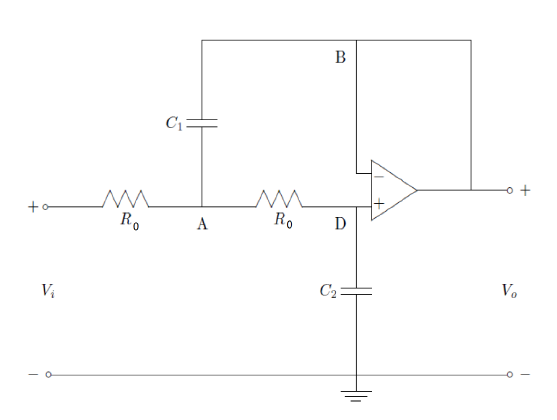
\includegraphics[scale=0.5]{P4.jpg}
\caption{Plant Circuit}
\end{figure}
Steps:
\begin{enumerate}
\item Construct the plant circuit according to Figure 4. Where $R_0=10k\Omega,C_1=100\mu F,C_2=0.22\mu F.$
\item Impulse response: A=1V, width=0.1s, f=1Hz. 
\item Step Response: A=1V, f=1Hz.
\end{enumerate}
For example, for the step response, you should try to get something like the waveform shown in following
gure.
\begin{figure}[H]
\centering
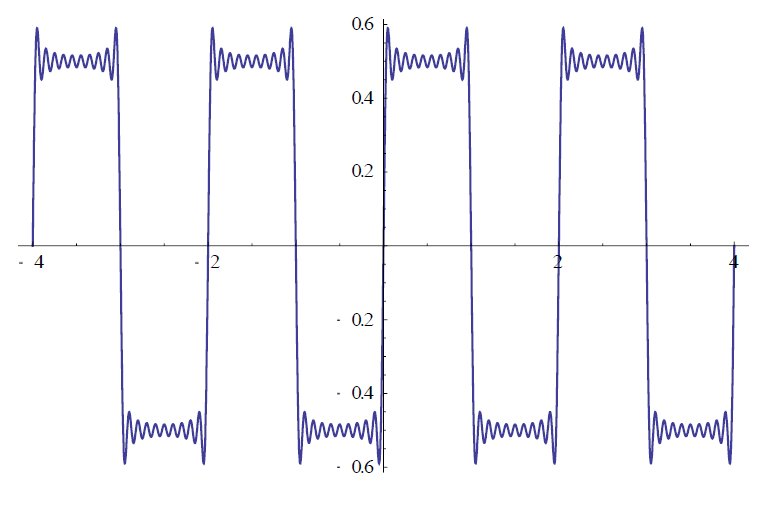
\includegraphics[scale=0.1]{P5.jpg}
\caption{Plant Result}
\end{figure}
\subsection{Feedback Control}
\begin{figure}[H]
\centering
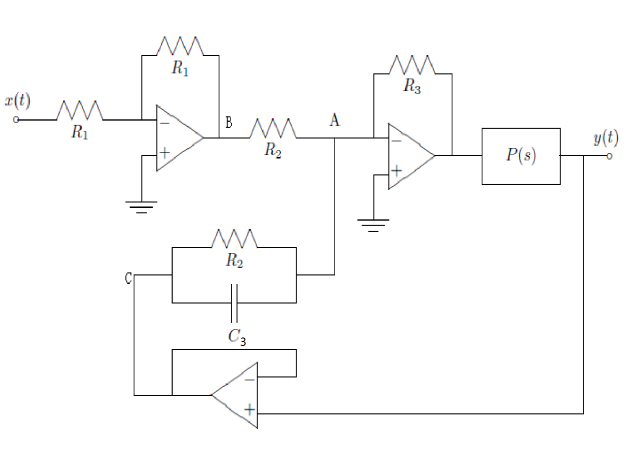
\includegraphics[scale=0.5]{P6.jpg}
\end{figure}
Steps:
\begin{enumerate}
\item Add the feedback control circuit to the plant according to Figure 5. Where $R1=R3=150k\Omega,R2=3k\Omega
,C3=0.47\mu F$.
\item Impulse response: A=1V, width=0.1s, f=1Hz.
\item Step Response: A=1V, f=1Hz.
\end{enumerate}
For example, for step response, you should try to get something like the waveform shown in the following
figure.
\begin{figure}[H]
\centering
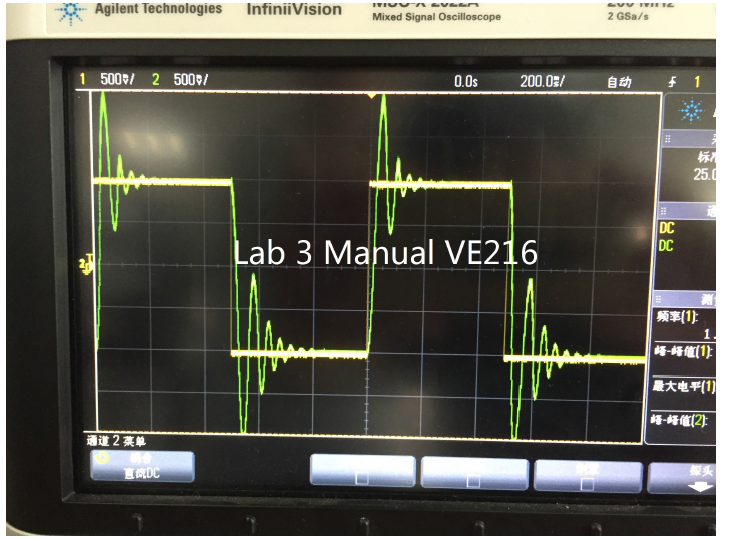
\includegraphics[scale=0.45]{P7.jpg}
\caption{Feedback Control Result}
\end{figure}
\section{Experiment Results}
\subsection{Open Control Plant}
\begin{figure}[H]
\centering
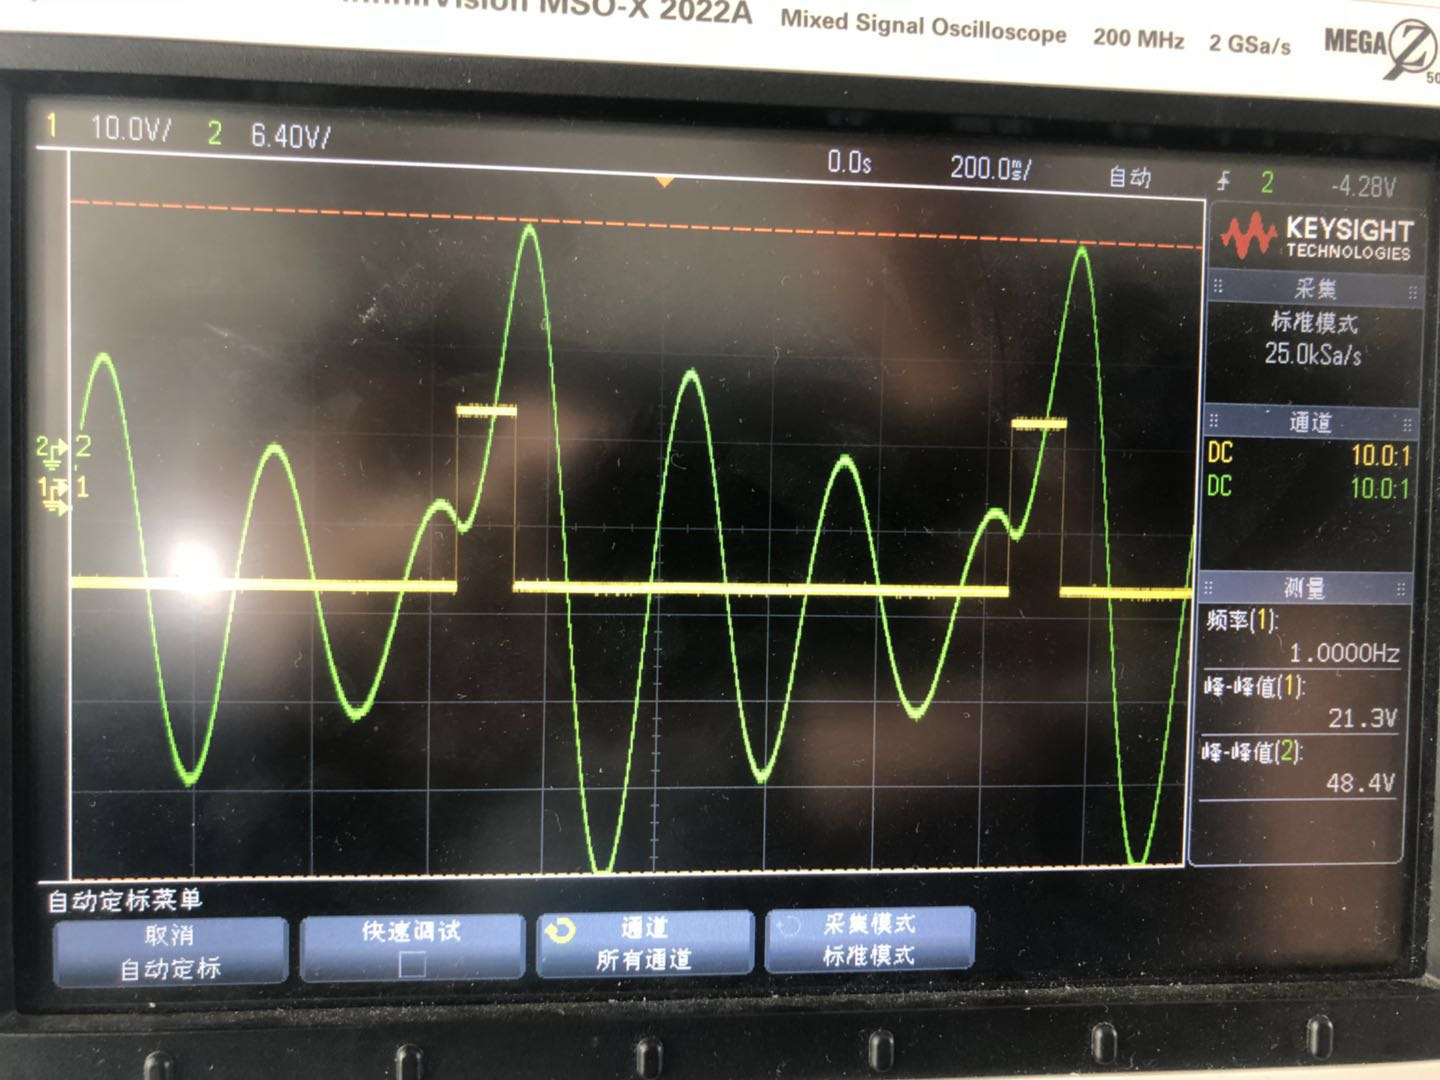
\includegraphics[scale=0.22]{P8.jpg}
\caption{Impulse Response}
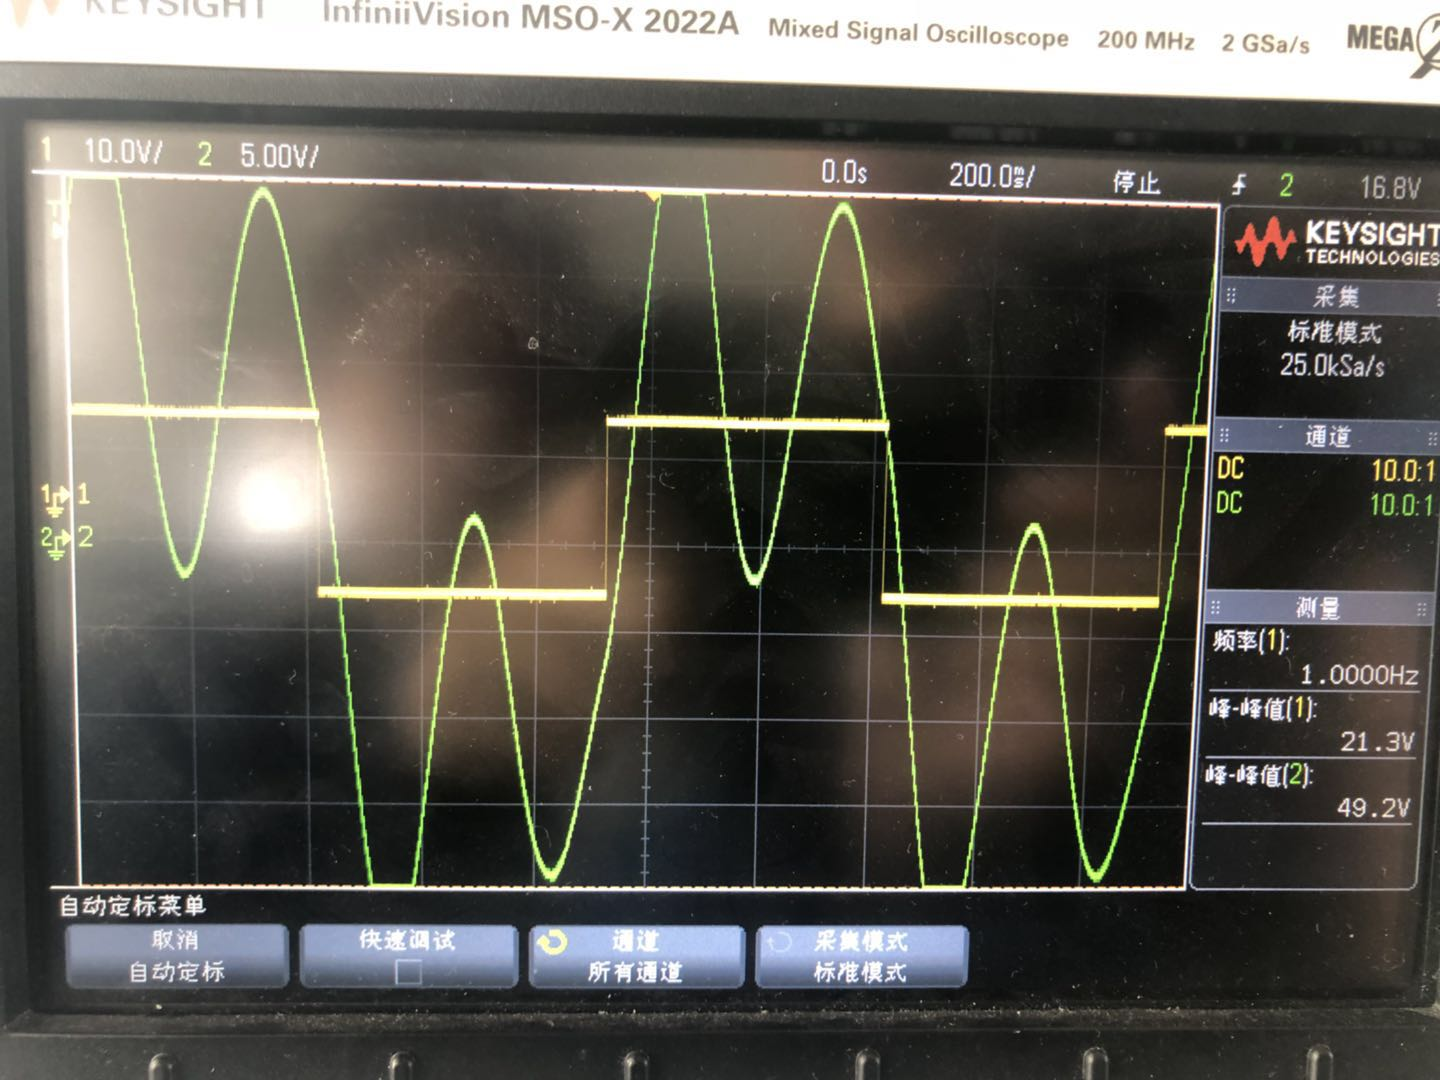
\includegraphics[scale=0.22]{P9.jpg}
\caption{Step Response}
\end{figure}
\subsection{Feedback Control}
\begin{figure}[H]
\centering
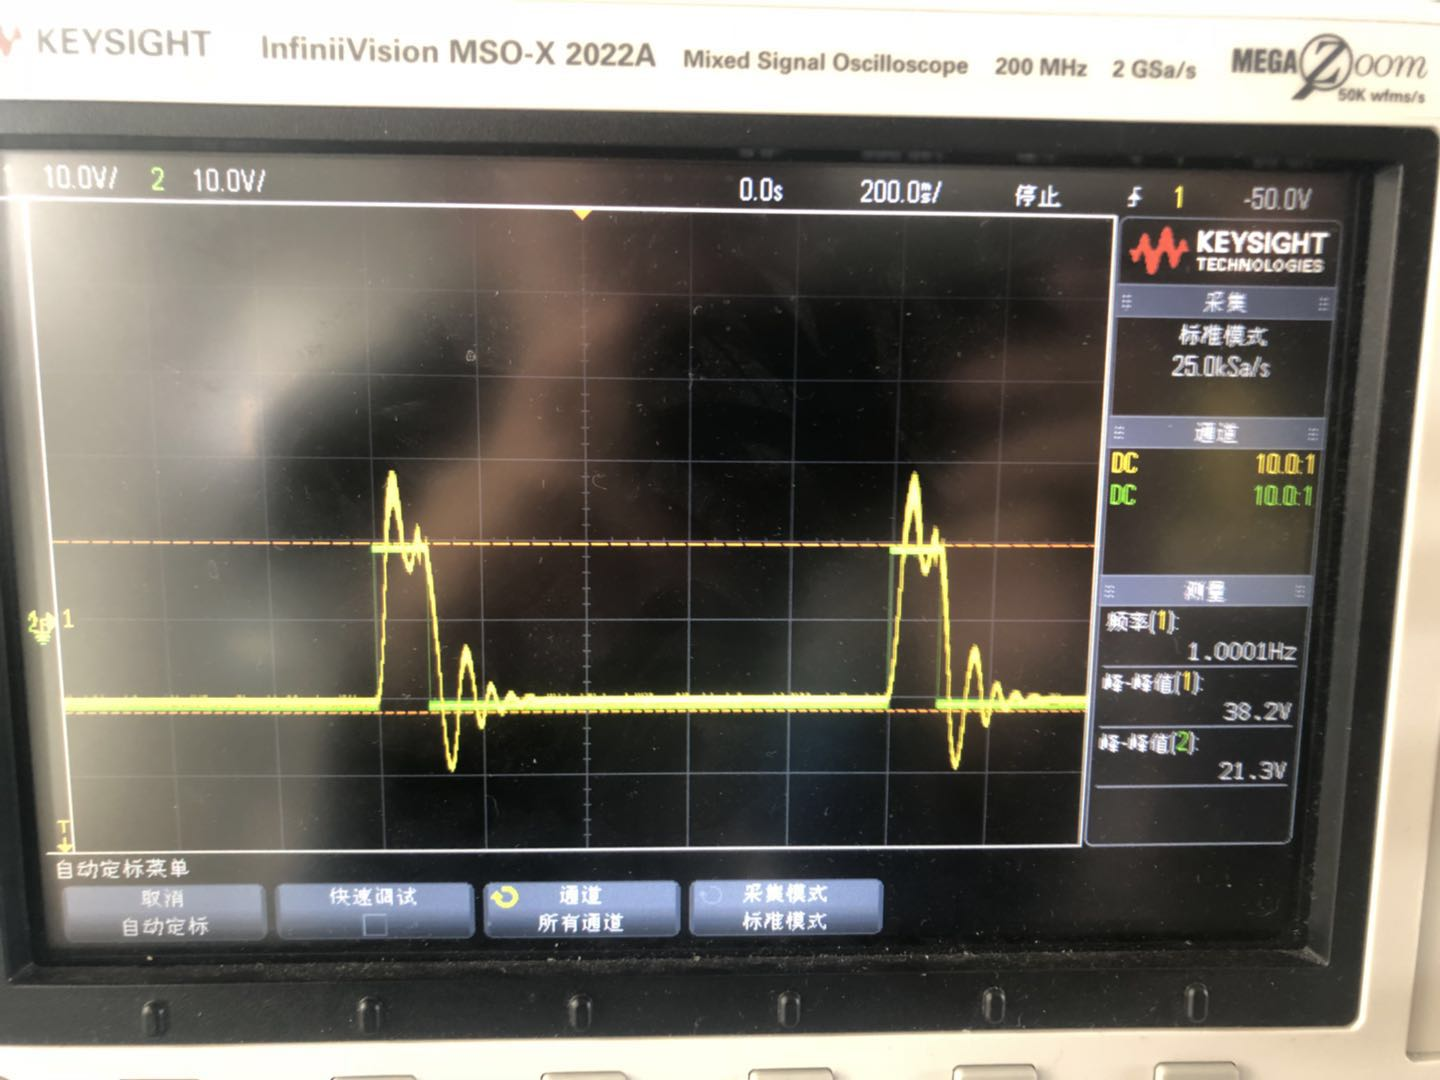
\includegraphics[scale=0.22]{P10.jpg}
\caption{Impulse Response}
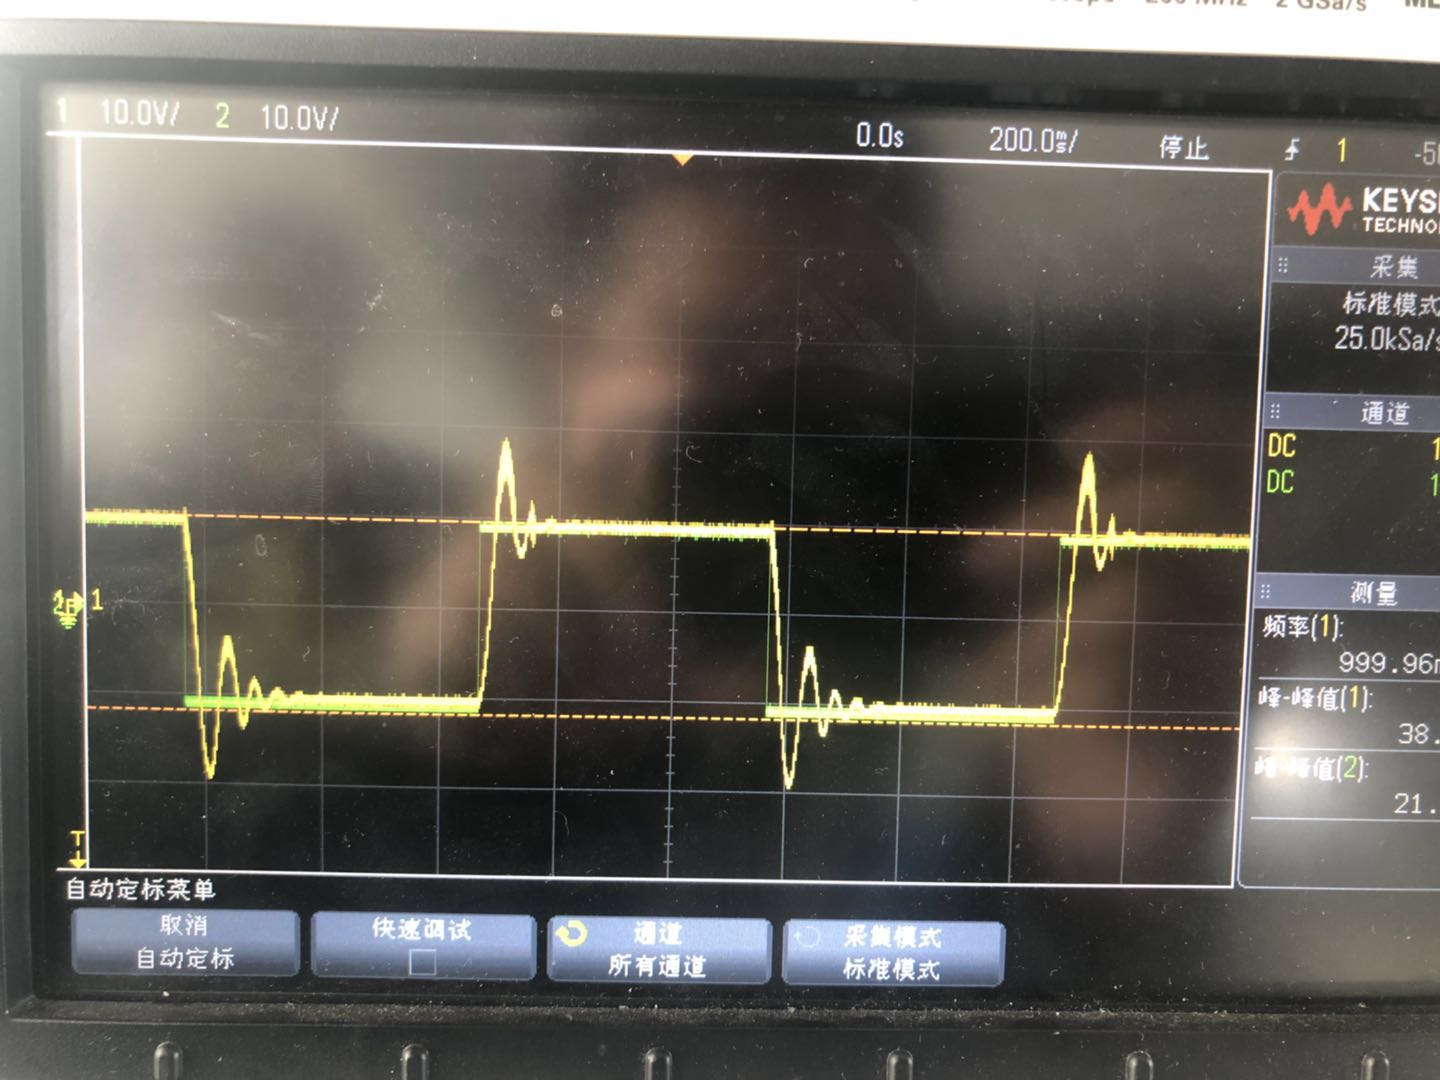
\includegraphics[scale=0.22]{P11.jpg}
\caption{Step Response}
\end{figure}
\section{Error Analysis and Discussion}
\subsection{Error Analysis}
In the first part of the lab, we were supposed to construct a Plant Circuit, which was the system whose output we wish to control in the whole feedback control system.
If we did it right, we were supposed to get the figure below, which was the case when the input signal was a square wave.
\begin{figure}[H]
\centering
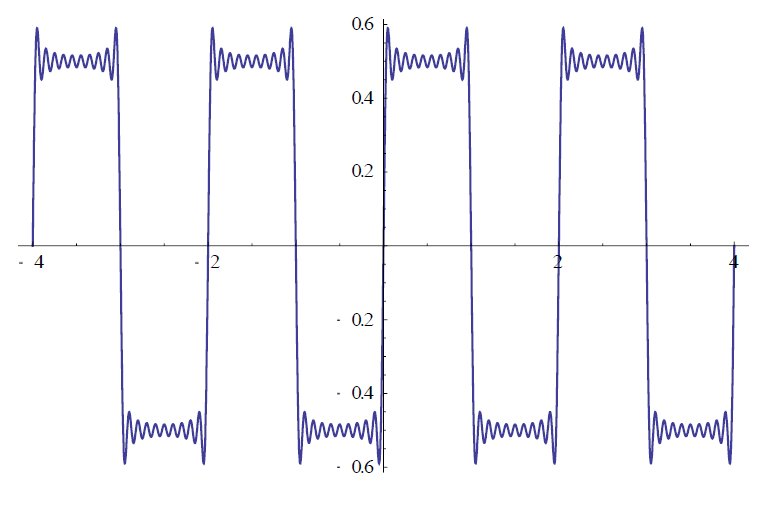
\includegraphics[scale=0.1]{P5.jpg}
\end{figure}
\begin{equation}
Y(s)=\frac{1/(C_1C_2R^2)}{s^2+(2/C_1R)s+1/(C_1C_2R^2)}
\end{equation}
\begin{equation}
Y(s)=\frac{1/(C_1C_2R^2)}{s^3+(2/C_1R)s^2+1/(C_1C_2R^2)S}
\end{equation}
Equation (27),(28) are the impulse response and step response in frequency domain respectively. According to prelab exercise, the two responses in time domain is 

\begin{equation}
\frac{1}{C_1 C_2 R^2}\cdot\frac{1}{2\sqrt{\frac{1}{C_1^2R^2}-\frac{1}{C_1C_2R^2}}}\cdot e^{-\frac{t}{C_1R}}(e^{\sqrt{\frac{1}{C_1^2R^2}-\frac{1}{C_1C_2R^2}}t}-e^{-\sqrt{\frac{1}{C_1^2R^2}-\frac{1}{C_1C_2R^2}}t})u(t)
\end{equation}
\begin{equation}
y(t)=(A_0+A_1e^{s_1t}+A_2e^{s_2t})u(t)
\end{equation}
\par And comparing to the ideal result, our figure was quite the same, which means that we did it correctly, and the error was neglectable.
\par In the second part of the lab, we would use the Plant Circuit we made in part 1 to make up a Feedback Control Circuit, and then we set the input signal as impulse signal and square wave signal to check the output. According to equation prelab assignment 3.5 
\begin{equation}
W(s)=K_p(X(s)-Y(s))-K_DsY(s)
\end{equation}
where W(s) is the input of P(s)
$$K_p=\frac{R_3}{R_2}=0.5\quad K_D=CR_3=0.0705$$
\par Also, if we did it right, we were supposed to get the figure below, which was the case when the input signal was a square wave.
\begin{figure}[H]
\centering
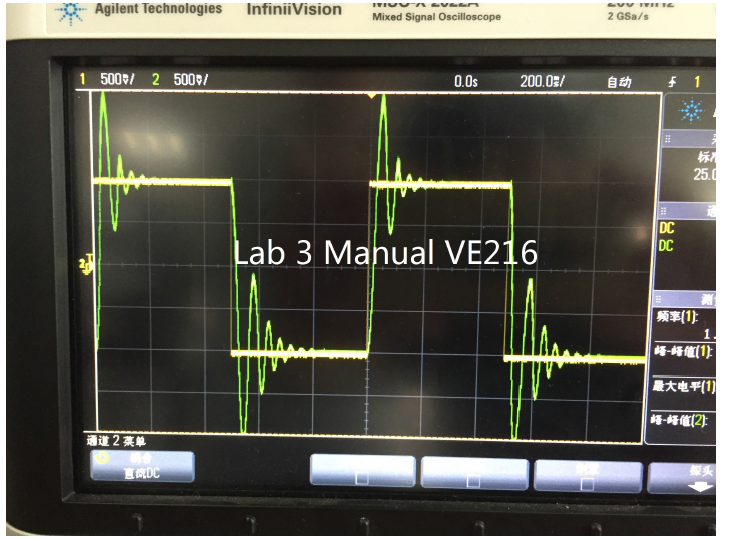
\includegraphics[scale=0.5]{P7.jpg}
\end{figure}
Comparing to the ideal result, our figure is quite the same, which means that we did it correctly and the error was neglectable. But during the lab, actually many groups’ figures had some “noises”, and also they did nothing wrong. And though in this lab, our group had no error or only the error that was neglectable, but we'll try to analyze the cause of the “noises” and something that you’d better be careful of.
\subsection{Discussion}
For the first part, actually at first, our group just burned the entire circuit, and we had to renew all the units. And the reason was that, we need a DC voltage to help the op amp work, but since the circuit was quite complex, we needed to use lots of wires, and when we were connecting the circuit, two wires just connected accidently, then the whole circuit was burned.
\par So we suggested that when we were connecting a complex circuit, you’d better use the long wires, and keep the nodes as separate as possible, it would help you see the circuit clearly and it could avoid short circuit.
\par And also, if you find your circuit is right, but you can’t get the right figure, you’d better check and change your units(like the capacitor, resistor), if you check and change the units, but it doesn’t work, then you’d better change your board.
\par For the second part, this circuit was far more complex than the first one, and since we burned the circuit in part 1, this time we were more careful, and we used lots of long wires to prevent us from making the same mistake.
\par And we think the reason why some groups’ figure had the “noises” was that: since the circuit is quite complex, sometimes you might let two wires cross each other. Since we had learned that the current will produce a magnetic field, and the changing magnetic field will also cause current. So the crossing wires might affect each other, then the “noises” appeared.
\par So, to prevent this phenomenon happened, we suggested that students should use long wire, and keep the nodes as separate as possible, and try to separate the crossing wires.
\section{Conclusion}
\subsection{Prelab}
We learned some basic knowledge about the Closed-Loop Feedback Model and Closed-Loop Transfer Function, and we know what is a Feedback Control System, and what’s the differences between different kinds of Control Systems.
\par By doing the Prelab assignments, we calculated the relationship between output and input of a Control System, so we can have a deeper understanding of the knowledge we learned before, and by using the matlab to draw the output figure, we got a general impression of the lab results.
\par We learned how to connect the circuit clearly and correctly, that is using long wire, and keeping the nodes as separate as possible.
\subsection{During the lab}
We did learn lots of things during the lab.It’s absolutely the most complex lab we have ever met. And since board had something wrong within it, it took us an hour to finish the first part. This “accident” did help us to improve our patience, and we learned the way to debug, that is check one layer at a time, when you find your circuit doesn’t work, don’t be nervous, just calm down, and first check the circuit, then check the units, then check the board, calm down and check it step by step, then you will figure it out. Also, by connecting the circuit ourselves and see the output figure, we had a deeper understanding of the basic concepts of the Feedback Control System.
\subsection{After the lab}
After the lab, we compared our results to the ideal results, and we were glad to find our results were very close to the ideal one, and by discussing with other teams, we analyzed the cause of the “noises”, and we review the relationship between current and magnetic field to solve this problem, so by doing this, we reviewed the knowledge we learned before and tried to use it to solve real problem, it improved our skills to apply knowledge to real life.
\par All in all, this lab is quite difficult but we finished it perfectly, and we not only learned new knowledge, but also review the old knowledge and improve ourselves in many aspects at the same time.
\par This lab is very interesting and helpful to us!

\end{document}